\chapter{Preprocesamiento de los datos cognitivos}

\section{Selección de los textos}

El corpus que se utilizó no solo para entrenar y mejorar la AWD-LSTM, sino también como base para los experimentos que generaron los datos cognitivos constó de una serie de 20 textos cortos (400 - 1500 palabras) seleccionados de diferentes fuentes literarias e informativas. La mayoría de ellos fueron extraídos del libro “100 covers de cuentos clásicos” de Hernán Casciari. Las historias originales fueron escritas por diversos autores, las cuales fueron simplificadas, traducidas en el caso de ser necesario y reescritas al español por Casciari. De esta manera, se persiste una diversidad en los estilos literarios, a su vez manteniendo tanto la dificultad como el uso de palabras autóctonas del dialecto rioplatense. El objetivo de esta selección es disponer de textos naturales (no diseñados específicamente para ser parte de este corpus), que puedan ser leídos en un tiempo de alrededor de 5 minutos cada uno, sin mayores inconvenientes, maximizando la cantidad de palabras únicas utilizadas. Es decir textos cortos de escritura amena. Además de la longitud, se tuvieron en cuenta sesgos culturales y de género en la selección del material, balanceando la presencia y las actividades de los y las protagonistas.

Para la selección de textos, se consideraron las restricciones impuestas por el procesamiento de las mediciones. Al procesar datos de experimentos de seguimiento ocular, es crucial tener en cuenta la pérdida de datos al eliminar fijaciones en los extremos de líneas y párrafos, ya que estas fijaciones no se asocian directamente con el procesamiento del texto. \parencite{Rayner1998} Por ello, se evitaron textos con muchas líneas cortas, oraciones breves o diálogos, que generan saltos de línea frecuentes. Además, para maximizar la utilidad del corpus comportamental, se priorizaron textos con baja proporción de palabras de muy baja frecuencia. \parencite{Inhoff1984}

\section{Experimentos de seguimiento ocular}

Los experimentos realizados se dividieron en sesiones independientes de hasta 1 hora, asegurando un nivel de atención adecuado. El participante se encargaba de realizar una prueba, donde debía leer uno de los cuentos del corpus separado en diversas pantallas, mientras se obtenían registros de los movimientos oculares (fijaciones) de la persona a medida que iba avanzando. Al participante se le permitía volver a leer fragmentos ya visitados o incluso volver a pantallas anteriores, con la idea de simular la lectura del cuento de la manera más real posible. Al finalizar, se hicieron preguntas para verificar la atención del mismo durante el experimento. Si el participante no respondía correctamente, se descartaba el texto o la sesión.

El registro de movimientos oculares se realizó con equipos \textit{EyeLink 1000} (SR Research, Ontario, Canadá) ya disponibles. Estos equipos poseen la mayor precisión temporal y espacial del mercado. Siguiendo las especificaciones del fabricante, se realizó una calibración del equipo antes y después de la lectura de cada texto. En esta se le pide al participante que fije la vista en determinados puntos en la pantalla. Sólo se aceptaron calibraciones/validaciones con un error promedio menor a 0.5 grados de ángulo visual. Luego, cada una de las sesiones fue analizada manualmente para verificar que los movimientos oculares sigan los patrones esperados y no haya descalibraciones severas. Durante estos análisis se tomaron ciertas libertades, por ejemplo, debido a que los datos de movimientos oculares suelen estar sujetos a descalibración en el eje y (filas), ocurrió que existieron varias fijaciones que se registraron por encima de las palabras en las que los ojos están enfocados. Dado este escenario, se estableció un umbral manual para definir las líneas (es decir, a qué línea de texto pertenece cada fila de fijaciones) en cada pantalla para cada prueba. De esta manera se reubicaron fijaciones mal asignadas para preservar el mayor número posible de fijaciones.

Luego, si la sesión del participante fue aceptada, se tenían en cuenta ciertos recaudos a la hora de descartar fijaciones:

\begin{itemize}
    \item Las fijaciones iniciales se descartaban si generaban regresiones, así como fijaciones extremadamente largas o cortas ($\sim1000 ms$ y $\sim50 ms$), ya que tienden a corresponder a momentos en los que el participante no está prestando atención o a detecciones incorrectas de fijaciones, respectivamente.
    \item En cada pantalla, y en cada línea se descartaron las primeras y últimas fijaciones automáticamente.
    \item Para cada línea, cualquier fijación regresiva entre la primera y la más a la izquierda se considera el resultado de alteraciones oculomotores (barridas de retorno) y se descartaban.
    \item Palabras que contienen cualquiera de los siguientes caracteres:

    \begin{center}
        ¿, ?, ¡, !, ., -, 1, 2, 3, 4, 5, 6, 7, 8, 9, 0
    \end{center}
\end{itemize}

Al finalizar las experimentaciones y su posterior preprocesamiento, se contaron con los siguientes datos:

\subsection{Métricas generales}
\bb{El total de participantes del experimento de seguimiento ocular ($N=76$) dió lugar a un total de 1126 peubas (\bb{[definir qué es una prueba]}). [Explicar de dónde salen las 110 pruebas descartadas].} Por lo tanto, se puede observar que para el entreno de la AWD-LSTM se contó con el 91,12\% de las pruebas que originalmente se recabaron \bb{quedándonos con un total de XXX pruebas (Tabla \ref{tab:metricas_generales}).}


\begin{table}[H]
    \centering
    \caption{\bb{[AGREGAR EPIGRAFE]}}
    \begin{tblr}{|>{\centering\arraybackslash}m{3cm}|>{\centering\arraybackslash}m{3cm}|>{\centering\arraybackslash}m{3cm}|>{\centering\arraybackslash}m{3cm}|}
        \hline
        Participantes & Pruebas & Pruebas descartadas & Pruebas finales \\
        \hline
        76 & 1126 & 110 & \bb{XXX}\\
        \hline
    \end{tblr}
    \label{tab:metricas_generales}
\end{table}

% \subsection{Cantidad de sujetos por cuento}
A partir de estos filtros se obtuvieron un promedio de $56,3$ pruebas por cada texto con un desvío estándar de $4,30$ pruebas  (Tabla \ref{tab:cuentos_pruebas}). Esto nos da la pauta de que los datos que fueron utilizados para entrenar el modelo de lenguaje están repartidos equitativamente en lo que a cuentos respecta.

\begin{scriptsize}
\begin{table}[H]
    \centering
    \caption{\bb{[HACER]}}
    \begin{tblr}{|>{\centering\arraybackslash}m{6cm}|>
    {\centering\arraybackslash}m{3cm}|>{\centering\arraybackslash}m{2cm}|}
        \hline
        Cuento & Autor & Pruebas \\
        \hline
        La noche de los feos & \bb{[HACER]}& 53 \\
        \hline
        Cómo funcionan los bolsillos & & 50 \\
        \hline
        La máscara de la Muerte Roja & & 53 \\
        \hline
        Las fotografías & & 50 \\
        \hline
        La salud de los enfermos & & 61 \\
        \hline
        Buenos Aires & & 54 \\
        \hline
        Wakefield & & 61 \\
        \hline
        Cómo funciona caminar en la nieve & & 50 \\
        \hline
        Ahora debería reírme, si no estuviera muerto & & 59 \\
        \hline
        El espejo & & 60 \\
        \hline
        Embarrar la magia & & 53 \\
        \hline
        La lluvia de fuego & & 61 \\
        \hline
        Educar para escalar y bucear & & 52 \\
        \hline
        El golpe de gracia & & 54 \\
        \hline
        La gallina degollada & & 60 \\
        \hline
        Rubí y el lago danzante & & 60 \\
        \hline
        La canción que cantábamos todos los días & & 60 \\
        \hline
        El almohadón de plumas & & 61 \\
        \hline
        Una rosa para Emilia & & 60 \\
        \hline
        La de la Obsesión por la Patineta & & 54 \\
        \hline
    \end{tblr}
    \label{tab:cuentos_pruebas}
\end{table}
\end{scriptsize}


\section{Generación de textos de entrenamiento}

Con todos los datos obtenidos a partir del corpus de texto y de los experimentos, se procedió a generar los textos de entrenamiento que se utilizaron para entrenar al modelo de lenguaje con el objetivo de notar una mejoría en su \textit{performance} y en la representación de sus \textit{embeddings} (Figura \ref{fig:pipeline}). En particular, se armaron 4 conjuntos de textos distintos para entrenar el modelo, diferenciándose en qué métrica se extrajo a partir de las fijaciones (en el caso de que se haya extraído alguna) hasta en la forma de generar el texto en sí.

\begin{figure}[htb]
    \centering
    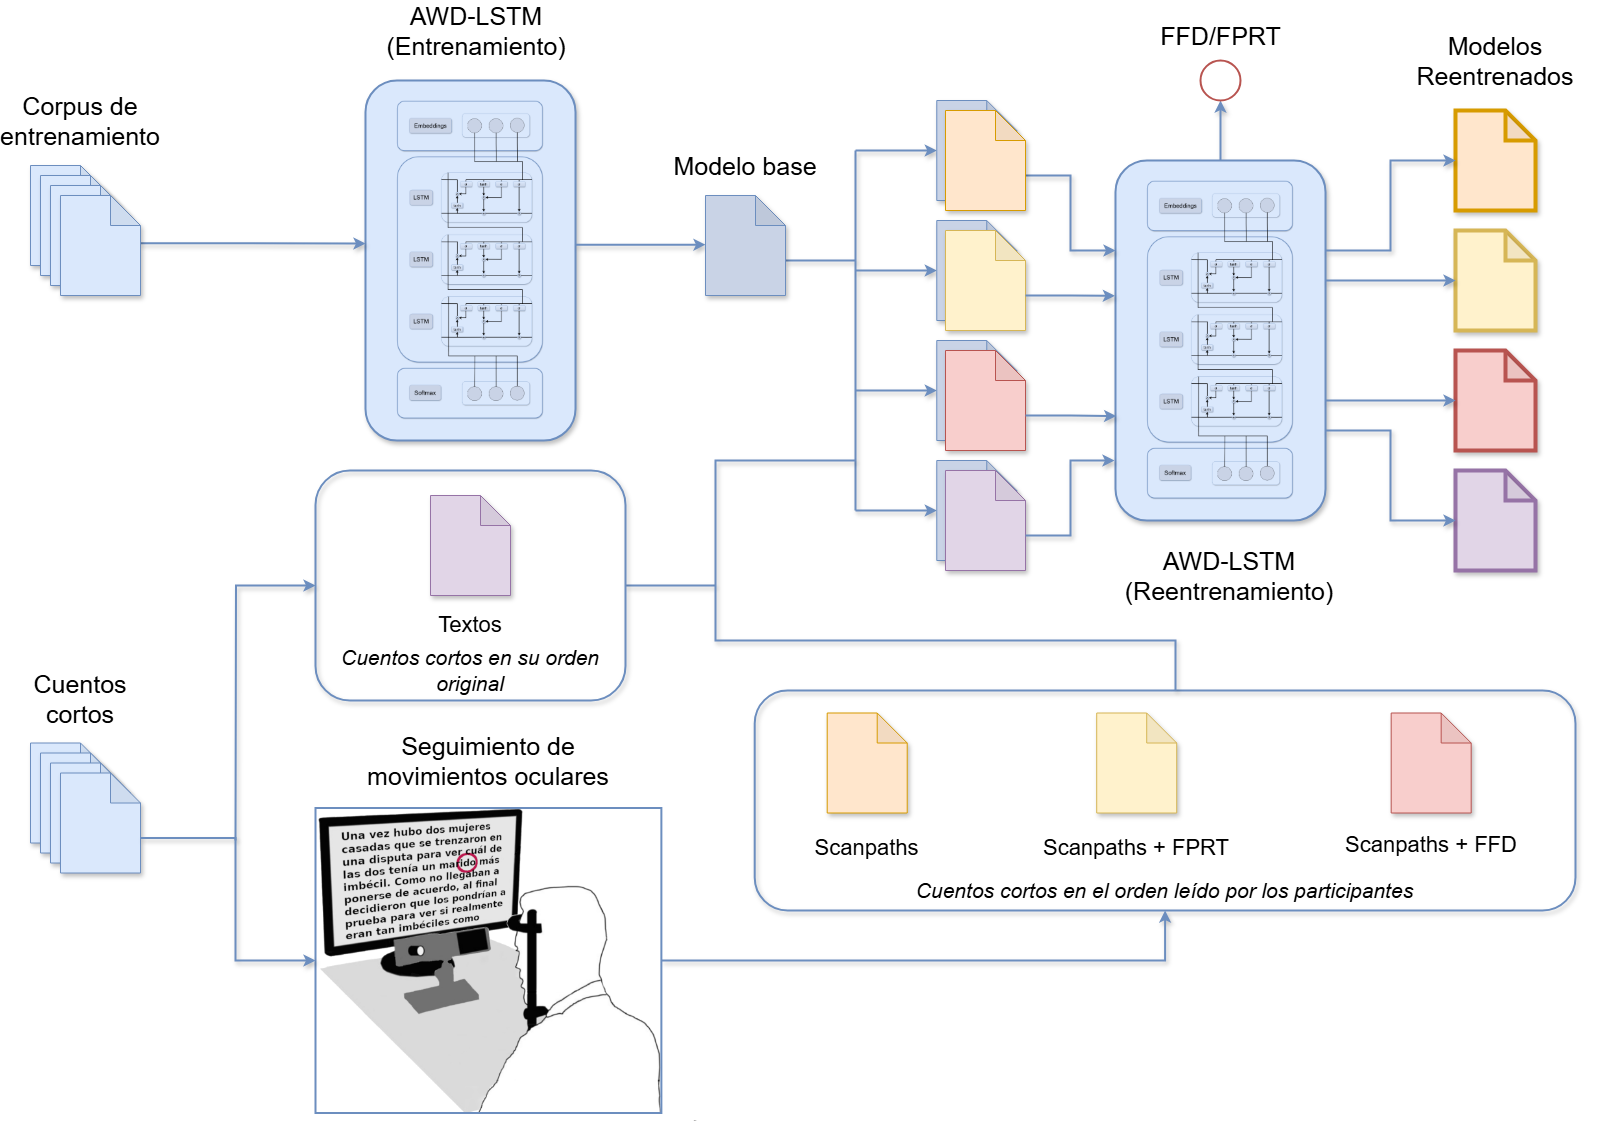
\includegraphics[width=1\textwidth]{imagenes/pipeline.png}
    \caption{Flujo de trabajo durante este proyecto. Se puede observar la generación de los textos basados en los cuentos acompañados con los movimientos oculares para reentrenar un modelo base}
    \label{fig:pipeline}
\end{figure}

\begin{enumerate}
    \item \textit{Textos}: En este caso directamente no se utiliza la información obtenida a partir de los experimentos y solamente se presentan los textos del corpus separados en 1 línea distinta por cada oración.
\end{enumerate}

Para los conjuntos restantes, se decidió utilizar como texto base los \textit{scanpaths} generados por los sujetos durante las pruebas. De esta manera, se puede tener una idea por sujeto de como fue realizándose la lectura de los cuentos. Ahora, para lograr que el modelo AWD-LSTM realice un mejor aprendizaje de las métricas extraídas de estos \textit{scanpaths}, debido a la variedad de valores entre un sujeto y otro, se tomó la decisión de asociar cada palabra dentro de los \textit{scanpaths} con el promedio de las métricas de todos los sujetos en vez de con el valor de la métrica para ese sujeto en particular. Con esto dicho, los conjuntos de reentrenamiento restantes fueron los siguientes:

\begin{enumerate}
    \setcounter{enumi}{1}
    \item \textit{Scanpaths}: Representación de los textos en formato \textit{scanpaths}, sin ninguna métrica en particular que lo acompañe. Por defecto, el valor de la métrica es reemplazado por un 0 para todas las palabras del \textit{scanpath}, pero no se aprende sobre ella.
    \item \textit{Scanpaths\_fprt}: Textos en formato \textit{scanpaths} utilizando la métrica \textit{Gaze Duration} o \textit{First Pass Reading Time}, donde se suman las duraciones de todas las fijaciones en una palabra (antes de salir hacia la derecha o la izquierda).
    \item \textit{Scanpaths\_ffd}: En este caso, los \textit{scanpaths} se ven influenciados por la métrica \textit{First Fixation Duration}, donde solo se conserva la primera fijación en una palabra (antes de salir hacia la derecha o la izquierda).
\end{enumerate}

El objetivo con estos textos es analizar el comportamiento del modelo al añadir información cognitiva, en particular, métricas tempranas sobre los movimientos oculares de los sujetos, las cuales están asociadas entre otras cosas, a la asociación semántica de las palabras.





